\begin{surferPage}[Barth-Sextic]{The Barth Sextic}
    %This surface of degree $6$ (sextic) was constructed by Wolf Barth in 1996.
		Ovu plohu stupnja $6$ (sekstiku) konstruirao je Wolf Barth 1996.
    
    %The Barth Sextic has $65$ singularities altogether.
		Barthova sekstika ima ukupno $65$ singulariteta.
%    (wenn man die $15$ im Bild nicht sichtbaren, ``unendlich fernen'', mitz�hlt)%
   %This is the maximum possible number of singularities on a sextic as shown
	Ovo je najve\'{c}i mogu\'{c}i broj singulariteta na sekstici, \v{s}to su pokazali
    %shortly after Barth's construction by Jaffe and Ruberman --- so, Barth's
    %world record is unbeatable!
		Jaffe i Ruberman nedugo nakon Barthove konstrukcije. Dakle, Barthov svjetski rekord je neoboriv!


    %Barth's construction was a big surprise because for a long time people
		Barthova konstrukcija bila je veliko iznena\dj{}enje jer se dugo mislilo da 
    %thought that surfaces of degree $6$ can only have $64$ singularities.
		plohe stupnja $6$ mogu imati samo $64$ singulariteta.

   %A striking feature of the construction is its icosahedral symmetry; 
	Iznena\dj{}uju\'{c}i dio konstrukcije je simetrija ikosaedra;
    %the figure shows an icosahedron and its symmetry planes:  
		figura predstavlja ikosaedar i njegove ravnine simetrije:
%    Die Abb.\ zeigt diesen platonischen K�rper und seine Symmetrie - Ebenen: 
%    und diese Ebenen gemeinsam mit der Barth Sextik in einem Bild.     
    % 
  \begin{center}
      \vspace*{-0.1cm}
      \begin{tabular}{@{}c@{\ \ }c@{\,}c@{}}
        \begin{tabular}{@{}c}
          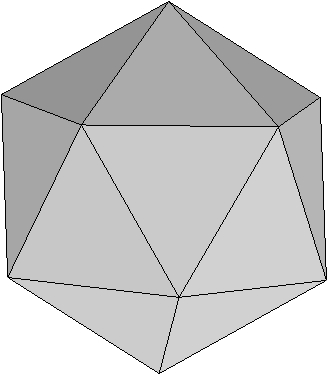
\includegraphics[width=1.4cm]{./../../common/images/icosah}
        \end{tabular}
        &
        \begin{tabular}{@{}c}
          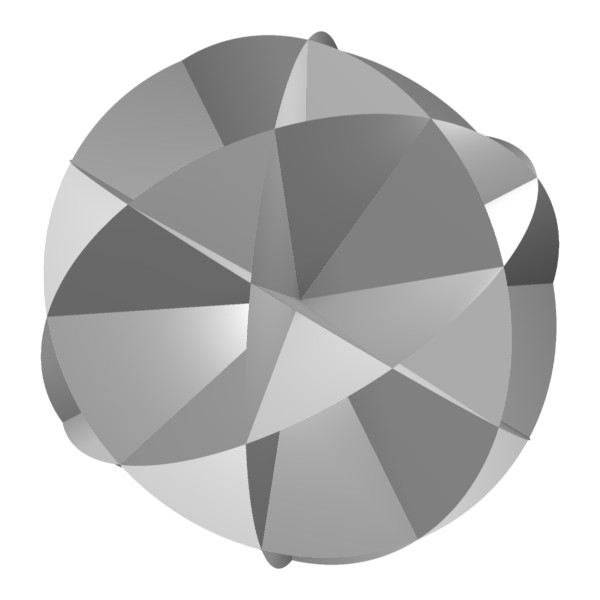
\includegraphics[width=1.4cm]{./../../common/images/barth_sextic_planes}
        \end{tabular}
        &
        \begin{tabular}{c@{}}
          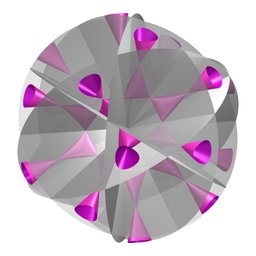
\includegraphics[width=1.4cm]{./../../common/images/barth_sextic_and_planes}
        \end{tabular}
      \end{tabular}
    \end{center}
    \vspace*{-0.1cm}

    %The Barth Sextic satisfies the equation 
		Barthova sekstika zadovoljava jednad\v{z}bu
    $P_6 - \alpha K^2=0,$
		%where
		gdje $P_6$
    %denote the 
		ozna\v{c}ava 
    %six symmetry planes, $K=x^2+y^2+z^2-1$ is the unit sphere and
		\v{s}est ravnina simetrije, $K=x^2+y^2+z^2-1$ je jedini\v{c}na sfera i 
    $\alpha=\frac{1}{4}(2+\sqrt{5})$.
\end{surferPage}
